\documentclass[11pt,a4paper]{article}
\usepackage[a4paper, left=3cm, right=2.5cm, top=2.5cm, bottom=2.5cm, headsep=1.5cm]{geometry}
\usepackage{graphicx}
\usepackage[T1]{fontenc}
\usepackage[polish]{babel}
\usepackage[utf8]{inputenc}
\usepackage{lmodern}
\usepackage{float}
\usepackage[figuresleft]{rotating}
\usepackage{multirow}
\usepackage{subfig}
\selectlanguage{polish}
\usepackage{makecell}
\usepackage{bytefield}
\usepackage{listings}
\def\code#1{\texttt{#1}}
\setlength{\parindent}{5mm}

\begin{document}
	\date{}
\begin{center}
	\centering


\includegraphics[width=4cm]{./rysunki/logo.jpg}
\\
\vspace{1.5cm}
 
\textbf{\Large POLITECHNIKA ŚLĄSKA}
\\
\vspace{0.5cm}
 
\textbf{\Large WYDZIAŁ AUTOMATYKI, ELEKTRONIKI}
\\
\vspace{0.1cm}
\textbf{\Large I INFORMATYKI}
\\
\vspace{0.5cm}


\vspace{3cm}
 
\textbf{\LARGE  Praca dyplomowa magisterska}
\\
\vspace{2cm}

\Large Implementacja SoC na podstawie mikroprocesora RISC-V Ibex
\vspace{3cm}

\begin{flushleft}
	
\Large Autor: inż. Dawid Zimończyk
\\
\Large Kierujący pracą: dr hab. inż. Robert Czerwiński, prof. Pol. Śl.
\\

\end{flushleft}
 \vspace{2.5cm}
\Large Gliwice, wrzesień 2020


\end{center}
\thispagestyle{empty}



\thispagestyle{empty}
\setcounter{page}{2}

\newpage

\begin{center}
\textbf {\Large Od autora}
\\
\vspace{0.5cm}

\newpage

\large\tableofcontents 

\newpage
\listoffigures
%\newpage
%\listoftables


\newpage

\textbf {\Large Spis ważniejszych oznaczeń}
\begin{flushleft}
SoC - System on Chip
\\ISA - instruction set architecture
\\RISC - Reduced Instruction Set Computing
\\UVM - Universal Verification Methodology
\\I2C - Inter-Integrated Circuit
\\SPI - Serial Peripheral Interface
\\UART - universal asynchronous receiver-transmitter
\\RAM - random-access memory
\\PWM - Pulse-Width Modulation
\\GPIO - general-purpose input/output
\\FPGA - field-programmable gate array
\\ISS - instruction set simulator
\\SV - SystemVerilog
\\DV - design verification
\\ISP - In-System Programming
\\JTAG - Joint Test Action Group
\\PC - program counter
\\LSB - least significant bit
\\MSB - most significant bit
\\IP - intellectual property
\\TLM - Transaction Level Modeling
\\DUT - Device under test
\\TCL - Tool Command Language
\\HDL - hardware description language
\end{flushleft}
\vspace{0.5cm}
\end{center}

\newpage
\section{Wprowadzenie} 

	\subsection{Wstęp}
	\hspace{5mm}
		\\
Systemy na chipie znane również jako SoC, występują w naszych telefonach czy samochodach. Również są częścią systemów wbudowanych, te zaś są wykorzystywane w każdej dziedzinie życia, od zegarków elektronicznych po zaawansowane roboty medyczne. Ważne jest więc by układy te były niezawodne i działały w zamierzony sposób. W celu weryfikacji działania układów, są wykorzystywane symulatory języków opisu sprzętu takie jak Riviera-PRO.
\\
\\
SoC powinien składać się z mikroprocesora, mikrokontrolera lub rdzenia DSP. Każdy mikroprocesor posiada 'Model programowy procesora' (ang Instruction Set Architecture, ISA). ISA definiuje jak mikroprocesor powinien działać, jego listę rozkazów, typ danych, tryby adresowania, rejestry dostępne dla programisty, zasady obsługi przerwań i wyjątków. Przykładowe komercyjne ISA: ARM, MIPS, Power ISA. Jest również otwarty model programowy procesora, który jest oparty o zasady RISC, jest nim RISC-V. Otwarta standard ISA oznacza, że dostęp nie jest limitowany prawnie, finansowo lub tajemnicą handlową firmy.
\newline
\newline
Przykładem mikroprocesora wykorzystującego ISA RISC-V jest Ibex. Jest on tworzony przez lowRISC, wywodzącego się z Uniwersytety w Cambridge. Mikroprocesor ten jest 32bit, składa się z 2-stage pipileine i został zaimplementowany na bazie RV32IMC.


	\subsection{Cel i zakres pracy}
	\hspace{5mm}
	\\
	Celem pracy jest implementacja SoC na podstawie mikroprocesora Ibex RISC-V. Mikroprocesor należy przystosować do implantacji na płytce FPGA NEXYS4DDR oraz dodać odpowiednie peryferia. Następnie przeprowadzić weryfikację zaimplementowanego systemu na chipie poprzez przeprowadzenie symulacji korzystając z biblioteki UVM 1.2 i testów RISCV complience. Weryfikacji zostanie poddany cały SoC jak i poszczególne peryferia.\newline
	Zakres pracy obejmuje:
	\begin{itemize}
	  \item Implementacje mikroprocesora IBEX
	  \item Implementacje peryferii:
	  \begin{enumerate}
	  	\item RAM
	  	\item SPI
	  	\item I2C
	  	\item UART
	  	\item GPIO
	  	\item Timer
	  \end{enumerate}
	  \item Kompilacja toolchaina i przystosowanie go dla SoC
	  \item Przeprowadzenie weryfikacji
  	  \item Porównanie wyników dla poszczególnych architektur i pamięci
  	  \item Podsumowanie wyników pracy
	\end{itemize}

	\subsection{Zarys pracy}
	\hspace{5mm}
	\\
	Praca składa się z 6 rozdziałów. Pierwszy zawiera krótkie omówienie tematu pracy, jej celu i zarys. Drugi rozdział jest poświęcony teorii. Opisuje on zagadnienia związane z ISA RISC-V, SoC, mikroprocesorem Ibex, kompilatorem, weryfikacją, płytce FPGA Nexys4 DDR i programem wykorzystanym do syntezy oraz programem do symulacji. Trzeci rozdział skupia się na implementacji poszczególnych części systemu na chipie, przedstawione zostaną w nim fragmentu opisu sprzętu, schematy blokowe i FSM. Czwarty rozdział przedstawia weryfikacje, opisuje przebiegające fazy biblioteki UVM 1.2 oraz jej wyniki. Następnie pokazuje symulację przeprowadzaną z instrukcjami wygenerowanymi przez RISCV-DV, Wyniki tej symulacji zostaną porównane z ISS Ovpsim i Spike. W piątym rozdziale zostaną porównane wyniki symulacji oraz syntezy architektury Von Neumanna z architekturą Harvardzką, pamięć RAM jedno-portowa z pamięcią RAM dwu-portową. Ostatni rozdział to podsumowanie oraz propozycję dalszego rozwoju projektu.
\newpage
	
\section{Część teoretyczna}

	\subsection{RISC V}

		\subsubsection{Instruction set architecture ISA}
		\hspace{5mm}
		\\
		RISC-V to otwarta ISA bazująca na architekturze RISC. Oznacza to, że licensja jest typu Open-source, która pozwala na wprowadzanie dowonlych modyfikacji\cite{open_source}, również jest nie wymaga żadnych opłat za wykorzystywanie jej w komercyjnych celach. Dokumentacja składa się z trzech części\cite{isa_site}:
		\begin{enumerate}
			\item User-Level ISA Specification - specyfikacja ISA poziomu użytkownika
			\item Privileged ISA Specifiation - specyfikacja ISA przywilejów
			\item Debug Specification - specyfikacja debugowania 
		\end{enumerate}
		Podstawowe cechy architektury RISC to:
		\begin{itemize}
		\item Zredukowana lista rozkazów, jest ich kilkadziesiąt
		\item Przepustowość procesora zbliżona do jednej instrukcji na cylk
		\item Zredukowana tryby adresowania, kody rozkazów są prostsze
		\item Powiększenie liczby rejestrów
		\item Minimalizacja komunikacja między procesorem a pamięcią
		\item Instrukcje mogą operować na dowolnych rejestrach
		\item Instrukcje zajmują w pamięci taką samą liczbę bajtów
		\item Procesor posiada architekturę Harwardzką
		\item Procesor używa przetwarzania potokowego
		\end{itemize}
		Są cztery podstawowe zestawy instrukcji oraz piętnaście ich rozszerzeń. W tabeli \ref{Tab:ISA} przedstawiono ich podział.
		\begin{center}
			\captionof{table}{ISA base and extensions\label{Tab:ISA}\cite{isa_book}}
			\begin{tabular}{|c|c|}
				\hline
				Nazwa  & Opis\\
				\hline
				\multicolumn{2}{|c|}{Podstawowe} \\
				\hline
				RV32I & Base Integer Instruction Set, 32-bit\\
				\hline
				RV32E & Base Integer Instruction Set (embedded), 32-bit, 16 registers\\
				\hline
				RV64I & Base Integer Instruction Set, 64-bit \\
				\hline
				RV128I & Base Integer Instruction Set, 128-bit \\
				\hline
				\multicolumn{2}{|c|}{Rozszerzenia} \\
				\hline
				M & Standard Extension for Integer Multiplication and Division \\
				\hline
				A & Standard Extension for Atomic Instructions \\
				\hline
				F & Standard Extension for Single-Precision Floating-Point \\
				\hline
				D & Standard Extension for Double-Precision Floating-Point \\
				\hline
				G & Shorthand for the base and above extensions \\
				\hline
				Q & Standard Extension for Quad-Precision Floating-Point \\
				\hline
				L & Standard Extension for Decimal Floating-Point \\
				\hline
				C & Standard Extension for Compressed Instructions \\
				\hline
				B & Standard Extension for Bit Manipulation \\
				\hline
				J & Standard Extension for Dynamically Translated Languages \\
				\hline
				T & Standard Extension for Transactional Memory \\
				\hline
				P & Standard Extension for Packed-SIMD Instructions \\
				\hline
				V & Standard Extension for Vector Operations \\
				\hline
				N & Standard Extension for User-Level Interrupts \\
				\hline
				H & Standard Extension for Hypervisor \\
				\hline
				\end{tabular}
		\end{center}https://riscv.org/specifications/
		Instrukcje są 32-bit. Tabela \ref{Tab:instruction} przedstawia formaty tych instrukcji. Korzystają one z sześciu formatów:
		\begin{itemize}
			\item Register (R) - instrukcje realizują działania na dwóch rejestrach {\it rs1} i {\it rs2}, wynik jest zapisywany w rejestrze {\it rd}.
			\item Immediate (I) - instrukcje realizują działania rejestrze {\it rs1} i liczbie 12bitowej stałej ze znakiem, wynik jest zapisywany w rejestrze {\it rd}.
			\item Upper immediate (U) - format wykorzystywany dla dwóch instrukcji: {\it LUI}, {\it AUIPC}. Służy do przypisywania liczb 20bitowych do rejestru {\it rd}.
			\item Store (S) - instrukcje realizują zapis do pamięci, pobierany jest bazowy adres z rejestru {\it rs1} + offset pochodzący z {\it imm}, rejestr {\it rs2} przechowuje.
			\item Branch (SB) - instrukcje realizują skoki warunkowe.
			\item Jump (UJ) - instrukcje służące do skoków, dodają wartość {\it imm} do {\it PC}.
		\end{itemize}
		\subsubsection{Rejestry}
		\hspace{5mm}
		\\RISC-V posiada 32 rejestry (tryb embeded posiada tylko 16). Jeśli korzystamy z rozszerzenia zawierającego liczby zmiennoprzecinkowe, dodane zostają kolejne 32 rejestry. Pierwszy rejestr nazywany jest rejestrem zerowym. Zawsze przyjmuje wartość zera, a wszystkie dane zapisywane do niego są tracone. Służy on jako rejestr pomocniczy w wielu instrukcjach.
		\pagebreak
		\begin{center}
			\captionof{table}{Rejestry RISC-V\label{Tab:registers}\cite{isa_book}}
			\nopagebreak[4]
			\scalebox{0.9}{\small
			\begin{tabular}{|c|c|c|c|}
			\hline
			Nazwa rejestry & Nazwa symboliczna& Opis & Właściciel \\
			\hline
			x0 & Zero & zawsze zero & \\
			\hline
			x1 & ra & adres powrotu &  wywołujący \\
			\hline
			x2 & sp & wskaźnik stosu & wołany (callee<?>) \\
			\hline
			x3 & gp & wskaźnik globalny & \\
			\hline
			x4 & tp & wskaźnik wątku & \\
			\hline
			x5 & t0 & \makecell{zmienna tymczasowa\\/ alternatywny adres powrotu} & wywołujący \\
			\hline
			x6-7 & t1-2& zmienne tymczasowe & wywołujący \\
			\hline
			x8 & s0/fp& zapisany rejestr / wskaźnik ramki & wołany \\
			\hline
			x9 & s1 & zapisany rejestr & wołany \\
			\hline
			x10-11 & a0-1 & argument funkcji / wartość zwracana & wywołujący \\
			\hline 
			x12-17 & a-2-7 & argument funkcji & wołany\\
			\hline
			x18-27 & s2-11 & zapisane rejestry & wołany \\
			\hline
			x28-31 & t3-6 & zmienne tymczasowe & wywołujący \\
			\hline
			\multicolumn{4}{|c|}{32 rejestry dla zmiennoprzecinkowego rozszerzenia} \\
			\hline
			f0-7 & ft0-7 & \makecell{tymczasowe zmienne \\ zmiennoprzecinkowe} & wywołujący \\
			\hline
			f8-9 & fs0-1 & \makecell{zapisane rejestry \\ zmiennoprzecinkowe} & wołany \\
			\hline
			f10-11 & fa0-1 & \makecell{argumenty/wartość zwaracana \\ zmiennoprzecinkowe} & wywołujący \\
			\hline
			f12-17 & fa2-7 & \makecell{argumenty \\ zmiennoprzecinkowe} & wywołujący \\
			\hline
			f18-27 & fs2-11 & \makecell{zapisane rejestry\\ zmiennoprzecinkowe} & wywołujący \\
			\hline
			f28-31 & fs8-11 & \makecell {tymczasowe zmienne \\zmiennoprzecinkowe} & wywołujący \\
			\hline
			\end{tabular}}
		\end{center}
		\begin{sidewaystable}
					\captionof{table}{32-bit RISC-V formaty instrukcji\label{Tab:instruction}\cite{isa_book}}
		\scalebox{0.9}{\small
			\begin{tabular}{*{33}{|c}|}
				\hline
              \multirow {2}{*}{Format} & \multicolumn{32}{c|}{Bit} \\
				\cline{2-33}
               & 31 & 30 & 29 & 28 & 27 & 26 & 25 & 24 & 23 & 22 & 21 & 20 & 19 & 18 & 17 & 16 & 15 & 14 & 13 & 12 & 11 & 10 & 9 & 8 & 7 & 6 & 5 & 4 & 3 & 2 & 1 & 0 \\
               \hline
               R & \multicolumn{7}{c|}{funct7}&\multicolumn{5}{c|}{rs2}&\multicolumn{5}{c|}{rs1}&\multicolumn{3}{c|}{funct3}&\multicolumn{5}{c|}{rd}&\multicolumn{7}{c|}{opcode}\\
               \hline
               I & \multicolumn{12}{c|}{imm[11:0]}&\multicolumn{5}{c|}{rs1}&\multicolumn{3}{c|}{funct3}&\multicolumn{5}{c|}{rd}&\multicolumn{7}{c|}{opcode}\\
               \hline
               U & \multicolumn{20}{c|}{imm[31:12]}&\multicolumn{5}{c|}{rd}&\multicolumn{7}{c|}{opcode}\\
               \hline
               S & \multicolumn{7}{c|}{imm[11:5]}&\multicolumn{5}{c|}{rs2}&\multicolumn{5}{c|}{rs1}&\multicolumn{3}{c|}{funct3}&\multicolumn{5}{c|}{imm[4:0]}&\multicolumn{7}{c|}{opcode}\\
               \hline
               SB & [12] & \multicolumn{6}{c|}{imm[10:5]}&\multicolumn{5}{c|}{rs2}&\multicolumn{5}{c|}{rs1}&\multicolumn{3}{c|}{funct3}&\multicolumn{4}{c|}{imm[4:1]}&[11]&\multicolumn{7}{c|}{opcode}\\
               \hline
               UJ & [20] & \multicolumn{10}{c|}{imm[10:1]}&[11]&\multicolumn{8}{c|}{imm[19:12]}&\multicolumn{5}{c|}{rd}&\multicolumn{7}{c|}{opcode}\\
               \hline
			\end{tabular}
			}
		\end{sidewaystable}
		
		\newpage

		\subsubsection{Dostęp do pamięci}
		\hspace{5mm}
			\\Dostęp do pamięci odbywa się za pomocą instrukcji {\it load/store}. W instrukcjach {\it load} adres bazowy znajduje się w rejestrze {\it rs1}, offset jest pobierany z liczby całkowitej 12bitowej {\it imm}. Rejestr docelowy znajduje się w {\it rd}. Przykład działania instrukcji {\it LW}:
			\begin{flushleft}			
			{\fontfamily{qcr}\selectfont
			lw x16, 8(x2)\\
			\begin{tabular}{*{5}{|c}|}
				\hline
				imm[11:0] & rs1 & func3 & rd & opcode\\
				\hline
				offset[11:0] & base\_addr & width & dst\_addr & LOAD\\
				\hline
				000000001000 & 00010 & 010 & 10000 & 0000011\\
				imm=+8 & rs1=2 & LW & rd=16  & LOAD\\
				\hline
			\end{tabular}
			}
			\end{flushleft}
			Wartość w {\it funct3} służy do dekodowania rozmiaru i znaku ładowanej wartości. Wartość ta jest zależna od użytego rozkazu, tabela \ref{Tab:load_instr} przedstawia zależność między instrukcją a wartością {\it func3}. 
			\begin{center}
			\captionof{table}{Zależność między {\it func3} a instrukcją load\label{Tab:load_instr}\cite{isa_book}}\small
				\begin{tabular}{|c|c|}
					\hline
					func3 & instrukcja \\
					\hline
					000 & LB \\
					\hline
					001 & LH \\
					\hline
					010 & LW \\
					\hline
					100 & LBU \\
					\hline
					101 & LHU \\
					\hline
				\end{tabular}
		\end{center}
		Kolejnymi instrukcjami są rozkazy {\it store}. Potrzebują one dwóch rejestrów, rejestr {\it rs1} zawiera bazowy adres pamięci, natomiast do rejestru {\it rs2} zostanie ona przypisana. Wartość offsetu jest pobierana z {\it imm}. Przykład działania instrukcji {\it SW}:
		\begin{flushleft}			
			{\fontfamily{qcr}\selectfont
			sw x16, 8(x2)\\
			\begin{tabular}{*{6}{|c}|}
				\hline
				imm[11:5] & rs2 & rs1& func3 & imm[4:0] & opcode\\
				\hline
				offset[11:5] & store\_addr & base\_addr & width & offset[4:0] & STORE\\
				\hline
				00000000 & 10000 & 00010 & 010 & 01000 & 0100011\\
				imm[11:0]=+8 & rs2=16 & rs1=2 & SW & & STORE\\
				\hline
			\end{tabular}
			}
			\end{flushleft}
			Podobnie jak w instrukcjach {\it load} func3 służy dekodowania rozmiaru i jest zależna od przekazanego rozkazu. Tabela \ref{Tab:store_instr} przedstawia tą zależność.
			\begin{center}
			\captionof{table}{Zależność między {\it func3} a instrukcją store\label{Tab:store_instr}\cite{isa_book}}\small
				\begin{tabular}{|c|c|}
					\hline
					func3 & instrukcja \\
					\hline
					000 & SB \\
					\hline
					001 & SH \\
					\hline
					010 & SW \\
					\hline
				\end{tabular}
		\end{center}
		\subsubsection{Instrukcje arytmetyczne i logiczne}
		\hspace{5mm}
			\\RISC-V zawiera zestaw instrukcji matematycznych przeznaczony dla liczb całkowitych w którego skład wchodzą: dodawanie, odejmowanie, przesuwanie , operacje logiczne i porównywanie liczb. Instrukcje dla mnożenia i dzielenia liczb znajdują się w rozszerzeniu ISA {\it M}. Zaś rozszerzenie ISA {\it F} zawiera instrukcje matematyczne dla liczb zmiennoprzecinkowych pojedynczej precyzji, rozszerzenie {\it D} zawiera instrukcje matematyczne dla liczb zmiennoprzecinkowych podwójnej precyzji\cite{isa_book}. Instrukcje te wykorzystują format {\it R} i {\it I}. Przykład działania rozkazu {\it add}, wykorzystuje on format instrukcji {\it R}:
			\begin{flushleft}			
			{\fontfamily{qcr}\selectfont
			add x6, x7, x8\\
			\begin{tabular}{*{6}{|c}|}
				\hline
				funct7 & rs2 & rs1 & func3 & rd & opcode\\
				\hline
				0000000 & 01000 & 00111 & 000 & 00110 & 0110011\\
				\hline
			\end{tabular}
			}
			\end{flushleft}
Pierwszy argument trafił to rejestru {\it rd}, kolejny do rejestru {\it rs1} ostatni do rejestru {\it rs2}. {\it Funct7} i {\it funct3} służą do rozpoznania operacji i są one zależne od przekazanej instrukcji. Tabela \ref{Tab:add_instr} przedstawia te zależności.
			\begin{center}
			\captionof{table}{Zależność między {\it func7} i {\it func3} a instrukcjami arytmetycznymi\label{Tab:add_instr}\cite{isa_book}}\small
				\begin{tabular}{|c|c|c|c|}
					\hline
					func7 & func3 & OPCODE & instrukcja \\
					\hline
					0000000 & 000 & 0110011 & ADD \\
					\hline
					0100000 & 000 & 0110011 & SUB \\
					\hline
					0000000 & 001 & 0110011 & SLL \\
					\hline
					0000000 & 010 & 0110011 & SLT \\
					\hline
					0000000 & 011 & 0110011 & SLTU \\
					\hline
					0000000 & 100 & 0110011 & XOR \\
					\hline
					0000000 & 101 & 0110011 & SRL \\
					\hline
					0100000 & 101 & 0110011 & SRA \\
					\hline
					0000000 & 110 & 0110011 & OR \\
					\hline
					0000000 & 111 & 0110011 & AND \\
					\hline
				\end{tabular}
		\end{center}
		Instrukcja {\it addi} wykorzystuje format {\it I}, więc trzeci argument rozkazu jest liczbą całkowitą. Przykład tej instrukcji: 
			\begin{flushleft}			
			{\fontfamily{qcr}\selectfont
			addi x6, x0, 50\\
			\begin{tabular}{*{5}{|c}|}
				\hline
				imm[11:0] & rs1 & func3 & rd & opcode\\
				\hline
				000000110010 & 00000 & 000 & 00110 & 0010011\\
				\hline
			\end{tabular}
			}
			\end{flushleft}
			{\it Func3} jest wykorzystywana w celu dekodowania instrukcji. Rozkazu przesunięcia bitowego wykorzystują pięć najmłodszych bitów z {\it imm}. Siedem pozostałych bitów służy do rozpoznawania instrukcji.
		\subsubsection{Instrukcje skokowe}
		\hspace{5mm}
			\\Instrukcje skokowe dzielą się na dwa rodzaje: skoki bezwarunkowe i skoki warunkowe. Pierwszą z nich reprezentują dwa rozkazy: \textit{JAL} (format \textit{UJ} i \textit{JALR} (format \textit{I}. Pierwszy z nich pozwala dodać do rejestru PC liczbę ze znakiem o szerokości 20bitów. Dzięki rozkazowi \textit{JALR} i \textit{AUIPC} można stworzyć skok o szerokości 32bitów. Rozkaz \textit{AUIPC} zapisuje do rejestru aktualną wartość PC, a rozkaz \textit{JALR}, zamienia dwanaście najmłodszych bitów na wartość przekazanego argumentu. Przykładowe programy z użyciem instrukcji skoków bezwarunkowych.
				\begin{lstlisting}[language=Ant]
addi x31, x0 ,0
auipc x2, 0
addi x31, x31, 1
addi x31, x31, 2
jalr x1, x2, 8
			\end{lstlisting}
			Program wpisuje do rejestru \textit{x2} aktualną wartość PC, następnie po wykonaniu dwóch instrukcji \textit{addi} następuje rozkaz\textit{jalr}, który dodaje wartość 8 do zapisanej wartości PC, więc kolejnym rozkazem wykonanym będzie \textit{addi x31, x31, 2}.
			\\
			Kolejną rodzajem są skoki warunkowe, jest ich sześć i są zakodowane w formacie \textit{SB}:
			\begin{itemize}
				\item BEQ - gdy zapisane liczby w rejestrach są równe wykonuje skok
				\item BNE - gdy zapisane liczby w rejestrach są różne wykonuje skok
				\item BLT - gdy liczba z rejestru \textit{rs1} jest większa wykonuje skok
				\item BLTU - gdy liczba z rejestru \textit{rs1} jest większa bądź równa wykonuje skok
				\item BHE - gdy liczba z rejestru \textit{rs2} jest większa wykonuje skok
				\item BGEU - gdy liczba z rejestru \textit{rs2} jest większa wykonuje skok
			\end{itemize}
	\subsection{System on Chip}

		\subsubsection{Architektura Harvardzka}
		\hspace{5mm}
			\\Architektura Harvardzka to rodzaj architektury komputera. Posiada ona dwie oddzielne szyny dla danych i rozkazów. Można w tym samym czasie pobierać argument wykonywanej funkcji i pobierać następnego rozkazu. Zwiększa ta szybkość pracy. Rysunek \ref{Fig:harvard} przedstawia schemat blokowy tej architektury.\\
\begin{samepage}
			\captionof{figure}{Schemat blokowy architektury Harvardzkiej\label{Fig:harvard}}
\nopagebreak
\begin{center}
		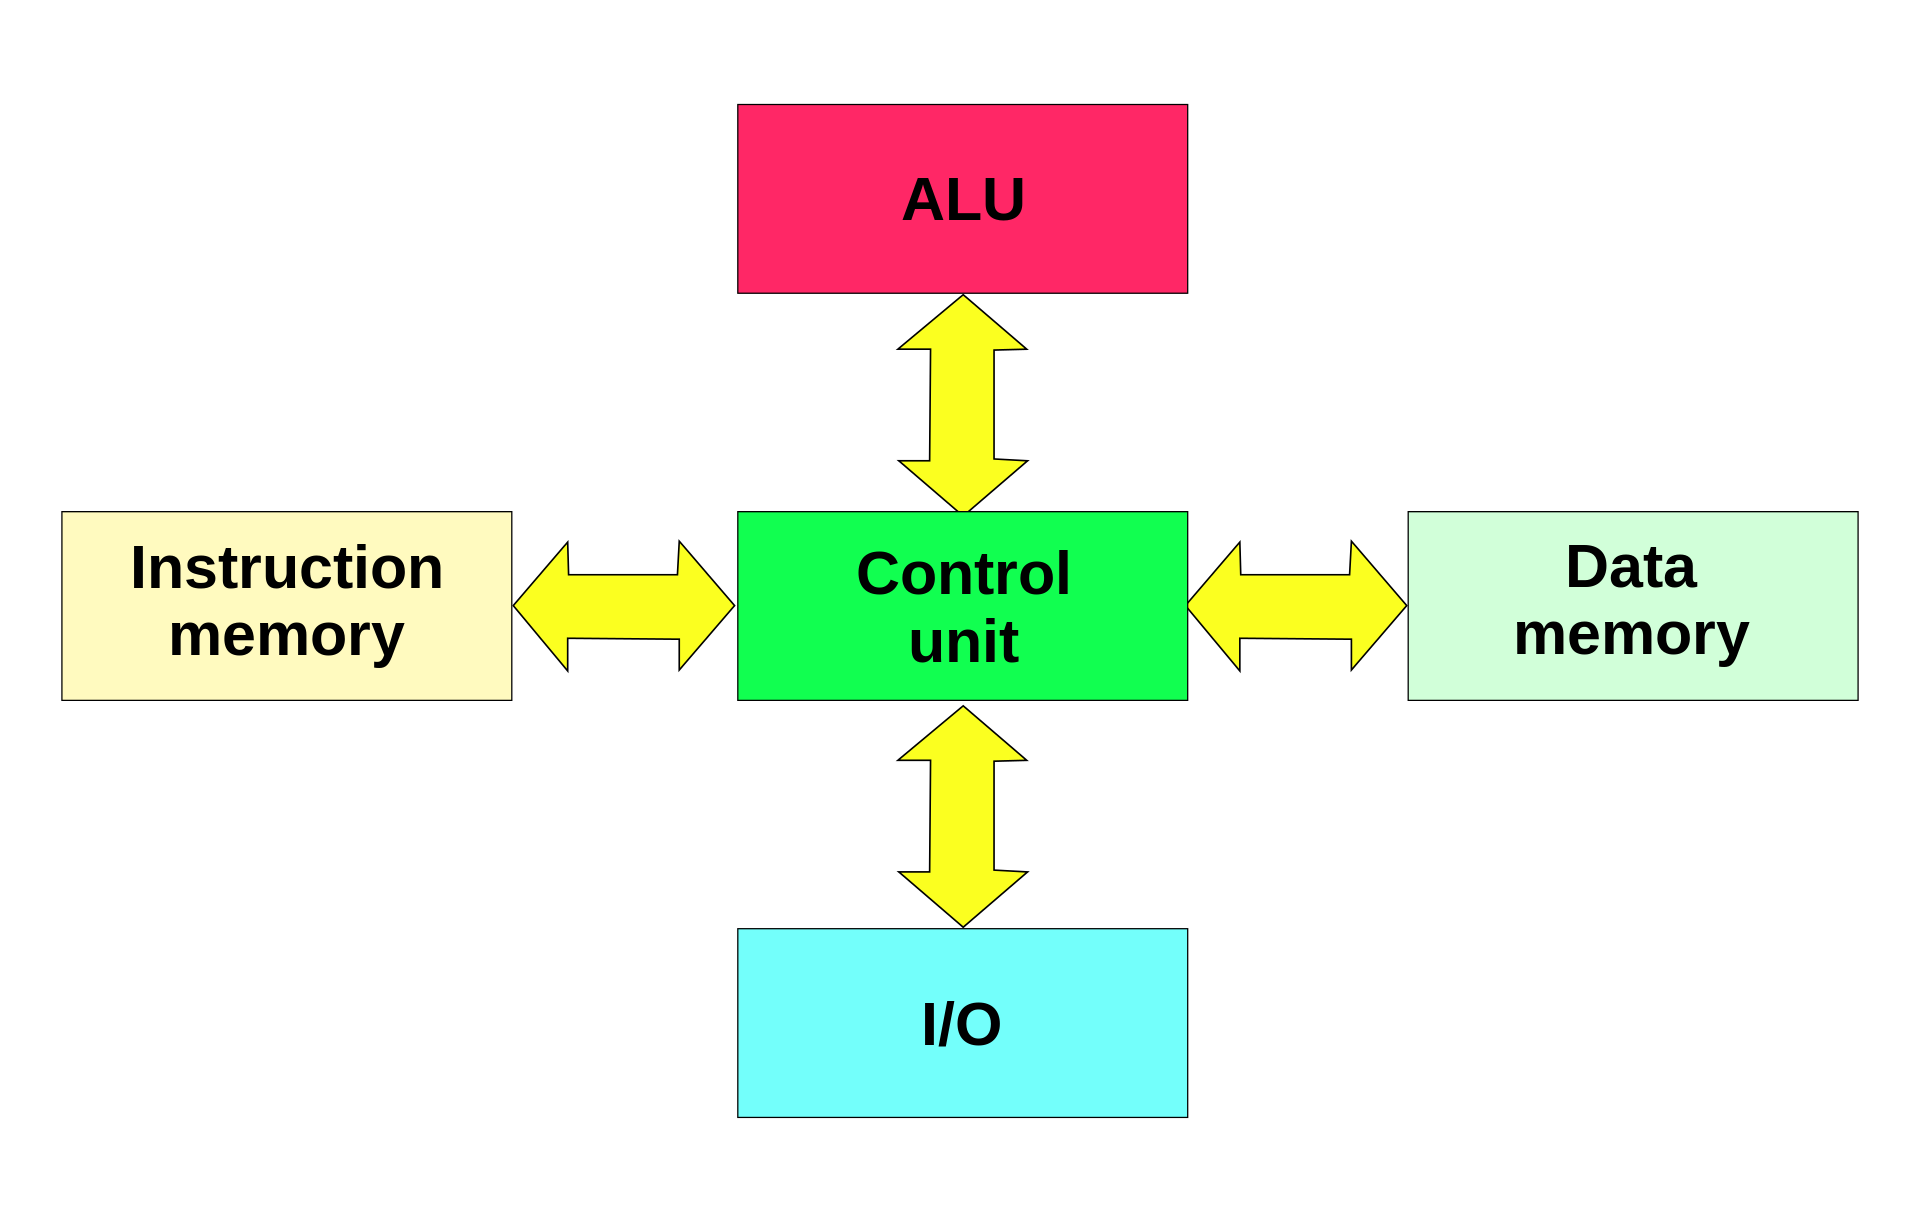
\includegraphics[width=10cm]{./rysunki/Harvard_architecture.png}
		\end{center}
\end{samepage}
		\subsubsection{Peryferia}
		\hspace{5mm}
			\\W projekcie zostały dodane następujące peryferia:
			\begin{enumerate}
			\item RAM - pamięć o dostępnie swobodnym, jest to podstawowy rodzaj pamięci cyfrowej. Może być ona odczytywana i zmieniana w dowolnej kolejności. Służy ona do przechowywania danych i kodu maszynowego. W projekcie zaimplementowano pamięć jedno-portową i dwu-portową. Pamięć jedno-portowa posiada tylko jeden dane/adres port, więc może być czytana lub zapisywana w jednej chwili czasu. Pamięć dwu-portowa zawiera dwa dane/adres porty, więc może być czytana i zapisywana w jednej chwili czasu.\cite{ram_book}
			\item SPI - interfejs służący do transmisji, głównie używany w systemach wbudowanych. Wykorzystuje się tryb \textit{master-slave}, dzięki temu jest zapewniona komunikacja full-duplex. Interfejs ten posiada następujące porty:
			\begin{itemize}
			\item $SCLK$ - zegar, wyjście z mastera.
			\item $MOSI$ - \textit{Master Out Slave In}
			\item $MISO$ - \textit{Master In Slave Out}
			\item $\overline{SS}$ - \textit{Slave Select}
			\end{itemize}
			 By rozpocząć transmisje, \textit{Master} konfiguruje \textit{SCLK}, następnie ustawia stan niski na \textit{SS} w celu wybrania odpowiedniego \textit{Slave'a}. \textit{Master} wysyła bit poprzez \textit{MOSI} i \textit{slave'a} odczytuje go i wysyła bit poprzez \textit{MISO}. Rysunek \ref{Fig:spi} obrazuję przebieg transmisji\cite{spi_book}.
			 \begin{samepage}
				\captionof{figure}{Przykład transmisji SPI\label{Fig:spi}}
				\nopagebreak
				\begin{center}
					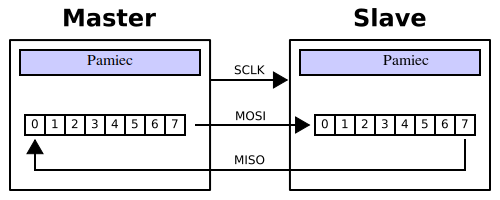
\includegraphics[width=13cm]{./rysunki/spi.png}
				\end{center}
			\end{samepage}
			
			\item I2C - magistrala szeregowa, dwukierunkowa, synchroniczna służąca do komunikacji. Wykorzystuje tryb \textit{master-slave}. Posiada dwa porty:
			\begin{itemize}
				\item SDA - Linia dla \textit{mastera} i \textit{slave'a} służąca do komunikacji między nimi
				\item SCL - linia przenosząca sygnał zegarowy
			\end{itemize}
			I2C może pracować z wieloma \textit{slave'ami} i \textit{masterami}. Rysunek \ref{Fig:i2c_frame} przedstawia wygląd ramki I2C. By rozpoacząć transmisje \textit{master} wysyła sygnał startowy. By to uzyskać sygnał na linii \textit{SDA} zmienia się z wysokiego na niski przed zmianą sygnały z wysokiego na niski na linii \textit{SCL}. Następnie jest przesyłany adres \textit{slave'a}. \textit{Slave} porównuje nadesłany adres i odsyła bit \textit{ACK} ustawiając na linii \textit{SDA} bit na stan niski. Po każdej udanej transmiji \textit{slave} przysyła \textit{masterowi} bit \textit{ACK}. W celu zakończenia transmisji należy w czasie wysokiego stanu \textit{SCL} zmienić stan z niskiego na wysoki na linii \textit{SDA}. Rysunek \ref{Fig:i2c_trans} przedstawia przykładowy przebieg transmisji.\cite{i2c_book}


			\item UART - urządzenie służące do asynchronicznej szeregowej komunikacji. Odbiera jak i wysyła informacje poprzez port szeregowy. Zawiera on on konwertery:
			\begin{itemize}
				\item szeregowo-równoległy - do konwersji danych wysyłanych do komputera
				\item równoległy-szeregowy - do konwersji danych pochodzących z komputera
			\end{itemize}	
			Rysunek \ref{Fig:uart_frame} przedstawia ramkę UARTu. Bit parzystości jest opcjonalny i służy jako bit kontrolny.\cite{uart_book}
			\begin{samepage}
				\captionof{figure}{Ramka UART\label{Fig:uart_frame}}
				\nopagebreak
				\begin{center}
					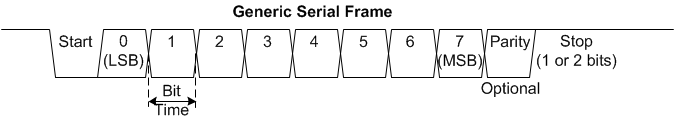
\includegraphics[width=13cm]{./rysunki/uart_frame.png}
				\end{center}
			\end{samepage}
			\item GPIO - piny służące do komunikacja między mikroprocesorem a peryferiami \cite{gpio_doc}
			\item Timer
			\end{enumerate}

		\subsubsection{Wishbone}
		\hspace{5mm}
			\\Wishobone to opensource magistrala służąca do łączenia ze sobą wielu IP w systemie \textit{master/slave}. Rysunek \ref{Fig:wishbone} przedstawia połączenia w tym interfejsie.
			\begin{samepage}
				\captionof{figure}{Wishbone master/slave interfejs\cite{wishbone_b4}\label{Fig:wishbone}}
				\nopagebreak
				\begin{center}
					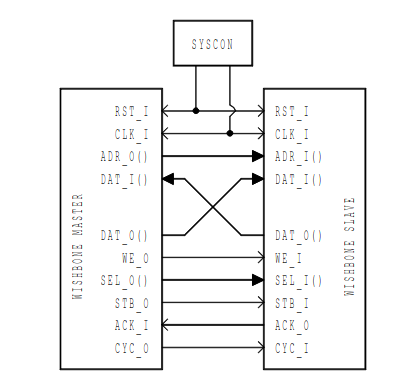
\includegraphics[width=10cm]{./rysunki/wishbone.png}
				\end{center}
			\end{samepage}
			Podczas implementacji tej magistrali należy trzymać się zasad które definiuje standard:
			\begin{itemize}
				\item Wszystkie sygnały interfejsu muszą być aktywne w wysokim stanie
				\item Wszystkie interfejsy \textit{WISHOBONE} muszą zainicjować siebie podczas asercji sygnału \textit{RST\_I}. Muszą zostać zainicjowane aż do narastającego zbocza \textit{CLK\_I}, której następuje po negacji \textit{RST\_I}.
				\item \textit{RST\_I} musi pozostać przynajmniej przez jeden pełny cykl zegarowy w stanie asercji.
				\item Wszystkie interfejsy \textit{WISHBONE} muszą być przygotowane na reakcję na \textit{RST\_I} w każdym momencie.
				\item \textit{RST\_I} może pozostać w stanie asercji dłużej niż jeden cykl zegarowy.
			\end{itemize}
			Porty używane przez ten interfejs\cite{wishbone_tutorial}:
			\begin{itemize}
				\item \textit{RST\_I} - sygnał resetu otrzymywany z \textit{SYSCON}
				\item \textit{CLK\_I} - sygnał zegarowy otrzymywany z \textit{SYSCON}
				\item \textit{ADR\_O/I} - linia adresu, wyjście z \textit{mastera}, wejście do \textit{slave'a}
				\item \textit{DAT\_I/O} - linia danych 
				\item \textit{WE\_O/I} - pozwolenie na zapis, wyjście z \textit{master}, wejście do \textit{slave}.
				\item \textit{SEL\_O/I} - selekcja bajtu, wyjście z \textit{master}, wejście do \textit{slave}.
				\item \textit{STB\_O/I} - potwierdzenie nadania danych przez \textit{mastera}, wyjście z \textit{master}, wejście do \textit{slave}.
				\item \textit{ACK\_I/O} - potwierdzenie przyjęcia danych przez \textit{slave'a}, wyjście z \textit{slave}, wejście do \textit{master}.
				\item \textit{CYC\_O/I} - cykl magistrali, wyjście z \textit{master}, wejście do \textit{slave}.
			\end{itemize}
			
		Są dostępne trzy topologie:
			\begin{enumerate}
				\item Data Flow Interconnection
				\item Crossbar Switch Interconnection
				\item Shared Bus Interconnection
			\end{enumerate}
			Ostatnia topologia została użyta w projekcie. Ma ona miejsce gdy wiele peryferii typu \textit{slave} jest podpięta do tych samych \textit{masterów}. Rysunek \ref{Fig:wishbone_sharedbus} przedstawia przykład tej topologii.
			\begin{samepage}
				\captionof{figure}{Wishbone shared bus interconnection\cite{wishbone_b4}\label{Fig:wishbone_sharedbus}}
				\nopagebreak
				\begin{center}
					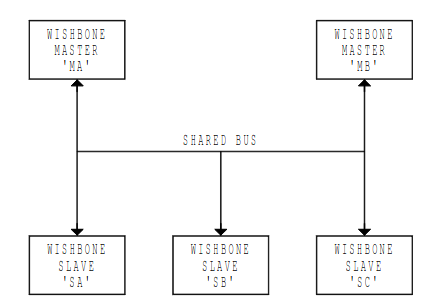
\includegraphics[width=10cm]{./rysunki/wishbone_sharedbus.png}
				\end{center}
			\end{samepage}
		W celu rozpoznania odpowiedniego \textit{slave'a} przypisuje im się adresy. Adresy te tworzą mapę, szczegółowy opis tejże mapy znajduje się w rozdziale 3.2.
	\subsection{Ibex}
	\hspace{5mm}
		\\Ibex jest to mikroprocesor tworzony przez organizację \textit{LowRISC}. Jest on dwupotokowy:
\begin{enumerate}
	\item Pobieranie instrukcji - pobiera instrukcje z pamięci.
	\item Dekodowanie i wykonanie instrukcji - zdekodowanie pobranej instrukcji i natychmiastowe jej wykonanie
\end{enumerate}		
		 Implementuje on \textit{ISA RV32IMC}. Wspiera on również rozszerzenie \textit{E} i eksperymentalne \textit{B}. Można je włączyć poprzez prawidłowe ustawienie parametrów\cite{ibex_doc}. Mikroprocesor ma szeroko rozwiniętą weryfikacje, wykorzystuje on między innymi generator rozkazów \textit{RISCV-DV}. Jest on również częścią projektu \textit{OpenTitan}, jest to \textit{RoT}, wspierany między innymi przez \textit{Google}\cite{google_opentitan}.
		Rysunek \ref{Fig:ibex_block} przedstawia schemat blokowy mikroprocesora \textit{Ibex}\cite{ibex_doc}.
			\begin{samepage}
				\captionof{figure}{Schemat blokowy mikroprocesora\label{Fig:ibex_block}}
				\nopagebreak
				\begin{center}
					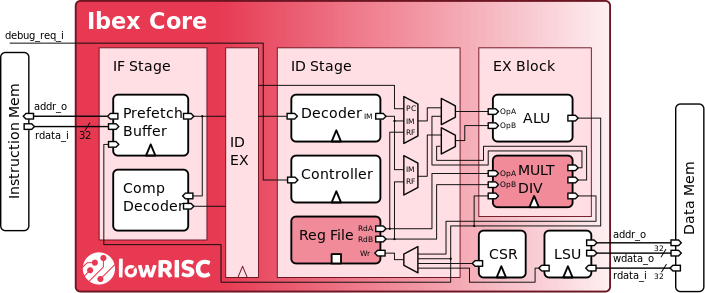
\includegraphics[width=14cm]{./rysunki/blockdiagram.png}
				\end{center}
			\end{samepage}
	\subsection{Kompilator}
		\subsubsection{Budowanie toolchaina}
		\hspace{5mm}
			\\Toolchain można pobrać z oficjalnego repozytorium \textit{RISC-V}\cite{toolchain}. By zbudować kompatibilną wersję kompilatora dla mikroprocesora \textit{Ibex}, należy do konfiguracji podać argumenty \textit{--with-abi=ilp32 --with-arch=rv32imc --with-cmodel=medany} lub skorzystać z \textit{--multilib}. Opcja ta spowoduje zbudowanie kompilatora dla 64bit, lecz po podaniu odpowiednich argumentów podczas kompilacji programu wspiera również architektury 32bit.
		\subsubsection{Przykładowa kompilacja}
		\hspace{5mm}
			\\By skompilować przykładowy program dla mikroprocesora 
			\textit{Ibex} należy użyć następujących komend: \\
\code{riscv32-unknown-elf-gcc -march=rv32imc -mabi=ilp32 -static -mcmodel=medany -nostdlib -nostartfiles -Wall -g -Os -MMD -c  -o led.o led.c
riscv32-unknown-elf-gcc -march=rv32imc -mabi=ilp32 -static -mcmodel=medany -nostdlib -nostartfiles -Wall -g -Os -MMD -c  -o crt0.o crt0.S
riscv32-unknown-elf-gcc -march=rv32imc -mabi=ilp32 -static -mcmodel=medany -nostdlib -nostartfiles -Wall -g -Os -T link.ld led.o crt0.o -o led.elf 
riscv32-unknown-elf-objcopy -O binary led.elf led.bin
srec\_cat led.bin -binary -offset 0x0000 -byte-swap 4 -o led.vmem -vmem
riscv32-unknown-elf-objdump -SD led.elf > led.dis
riscv32-unknown-elf-objcopy -O verilog --interleave-width=4 --interleave=4 --byte=0 led.elf led.hex} ŁADNIE TO ZROBIĆ\\
Pierwsze dwie komendy tworzą biblioteki, trzecia komenda spaja ze sobą potrzebne biblioteki i konsolidatora i tworzy plik \textit{bin}. Następnie plik \textit{bin} jest konwertowany do plików \textit{vmem} i \textit{hex}.
	\subsection{Weryfikacja}

		\subsubsection{UVM}
		\hspace{5mm}
			\\UVM jest to biblioteka oparta na języku \textit{SystemVerilog} służąca do tworzenia testów weryfikacyjnych. UVM zawiera bazowe klasy z metodami, które pomagają w weryfikacji. Ważniejsze klasy bazowe biblioteki:
			\begin{enumerate}
				\item uvm\_object - podstawowa klasa bazowa, zawierająca metody: \textit{create, copy, clone, compare, print, record}. Zazwyczaj używana do budowy testbenchu i konfiguracji testcase'u
				\item uvm\_component - wszystkie komponenty testbenchu takie jak \textit{scoreboards, monitor, driver} pochodzą z tej klasy.
				\item uvm\_sequence - jest klasą bazową wszystkich sekwencji zawartych w testbenchu
			\end{enumerate}
UVM test składa się z następujących elementów:
\begin{itemize}
	\item UVM test - jest odpowiedzialny za konfigurację testbenchu, rozpoczęcie symulacji poprzez inicjalizację sekwencji, stworzenie wszystkich komponentów, której znajdują się poniżej w hierarchii na przykład: uvm\_env.
	\item UVM env - grupuje agentów i scoreborady
	\item UVM Agent - łączy ze sobą \textit{uvm\_components} na przykład:\textit{uvm\_driver, uvm\_monitor, uvm\_suquence, uvm\_sequencer} za pomocą interfejsów TLM.
	\item UVM Driver - jest odpowiedzialny za wysyłanie pakietów do DUT
	\item UVM Sequence - generuje pa kiety
	\item UVM Sequencer - jest odpowiedzialny za ruch między \textit{uvm\_sequence} i \textit{uvm\_driver}
	\item UVM Monitor - obserwuje sygnały, następnie wysyła je do \textit{uvm\_scoreboard}
	\item UVM Scoreboard - odbiera dane z \textit{uvm\_monitor} i porównuje z spodziewanymi wartościami. Wartości te mogą pochodzić z modelu referencyjnego lub \textit{golden pattern}.
\end{itemize}
		Rysunek \ref{Fig:uvm_block} przedstawia przykładowy graf UVM testu
					\begin{samepage}
				\captionof{figure}{Przykładowy graf UVM\label{Fig:uvm_block}}
				\nopagebreak
				\begin{center}
					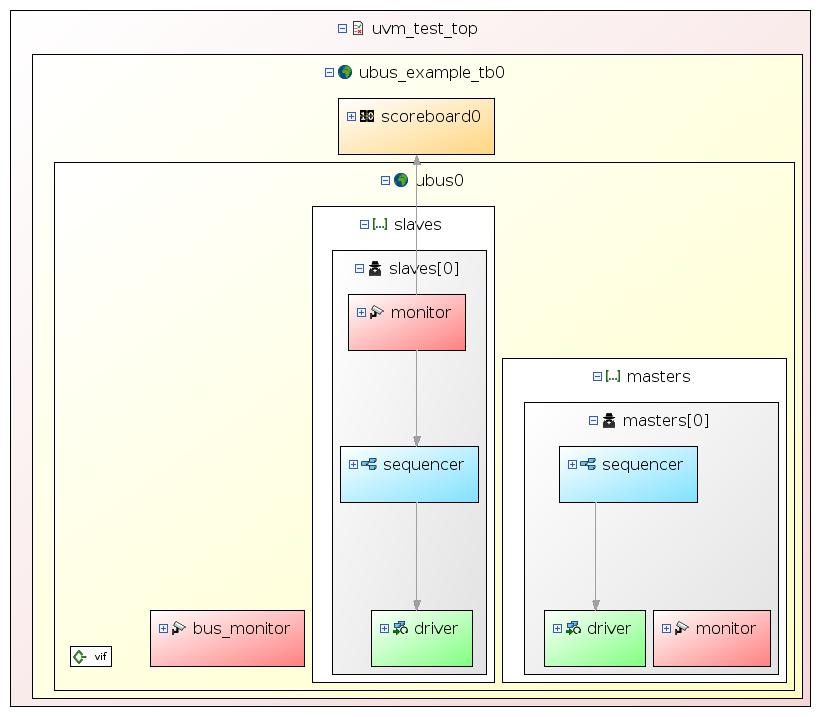
\includegraphics[width=14cm]{./rysunki/uvm_graph.jpg}
				\end{center}
			\end{samepage}
		\subsubsection{RISCV DV}
		\hspace{5mm}
			\\RISCV-DV - narzędzie/IP służące do generacji programów w języku assembler do testowania danych aspektów procesora. Współpracuje z ISA: \textit{RV32IMAFDC, RV64IMAFDC}. Programy są tworzone losowo. By korzystać z tego nardzędzia/IP należy posiadać symulator wspierający UVM, na przykład: Riviera-PRO \cite{google_dv}.

	\subsection{FPGA}
	\hspace{5mm}
		\\SoC będzie działać na płytce NEXYS4 DDR wyposażony w programowalny układ logiczny Artix-7 XC7A100T-1CSG324C. Ważniejsze zasoby płytki:\cite{nexys}
		\begin{itemize}
			\item 15850 plastrów logicznych, każdy złożony z czterech elementów LUT o 6-wejściach i 8 przerzutników
			\item Pojemność 4860 kb szybkiego bloku pamięci RAM
			\item Sześć bloków zarządzania sygnałem zegarowym (CMT), każdy z pętlą fazową (PLL)
			\item 240 plastrów DSP
			\item 16 przełączników użytkownika
			\item Mostek USB-UART
			\item Port USB-JTAG Digilent do komunikacji i programowania FPGA
			\item Cztery porty Pmod
		\end{itemize}

	\subsection{SystemVerilog}
	\hspace{5mm}
		\\Język opisu sprzętu, jest rozszerzeniem języka Verilog. Dodaje on nowe typy danych: \textit{logic, enum, byte, shortint, int, longint, struct, union}, wielowymiarowe tablice. Dodano również nowe bloki proceduralne: \textit{always\_comb, always\_latch, always\_ff}. Wprowadzono interfejsy wraz z \textit{modportami}, pomagają one zapanować nad portami w projekcie. Udoskonalono weryfikację poprzez dodanie nowego typu danych: \textit{string}, klas, asercji oraz \textit{constrained random generation} pozwalający narzucić ograniczenia podczas randomizacji.\cite{SV}
			
			\subsubsection{Xilinx Vivado Design Suite}
			\hspace{5mm}
				\\Vivado Design Suite - oprogramowanie firmy Xilinx dla syntezy i analizy projektów HDL. Posiada wbudowany symulator \textit{ISIM} oraz \textit{Vivado IP Integrator} pozwalający na szybkie zarządzanie IP.
				
			\subsubsection{Aldec Riviera-PRO}
			\hspace{5mm}
				\\Riviera-PRO komercyjny symulator HDL firmy Aldec. Obsługuje on bibliotekę UVM, randomizacje, asercje oraz może być wykorzystany do generacji programów assembler w celu weryfikacji działania SoCa.
				
\newpage

\section{Implementacja}

	\subsection{Ibex}
	\hspace{5mm}
		\\Głównym modułem jest \textit{ibex\_core}. By poprawnie działał z magistralą \textit{Wishbone}, należy opisać \textit{wrapper} w odpowiedni sposób. W tym celu powstał moduł \textit{ibex\_wb}, jego zadaniem jest poprawne przeniesienie sygnałów do interfejsów magistrali \textit{Wishbone}. Moduł ten został zainicjowany w module nadrzędnym \textit{ibex\_soc}. Moduł ten zawiera w sobie instancje wszystkich peryferii jak również interfejsów magistrali \textit{Wishbone}.

	\subsection{Wishbone}
	\hspace{5mm}
		\\opis interfejsów które dodałem, jak działa sharebus, połączenia między wszystkim
		
	\subsection{RAM}
	\hspace{5mm}
		\\cos o ram

	\subsection{GPIO}
	\hspace{5mm}
		\\opis gpio

	\subsection{UART}
	\hspace{5mm}
		\\opis uart

	\subsection{I2C}
		\subsubsection{master}
		\hspace{5mm}
			\\opis i2c master
		\subsubsection{slave}
		\hspace{5mm}
			\\opis i2c slave

	\subsection{SPI}
		\subsubsection{master}
		\hspace{5mm}
			\\opis spi master
		\subsubsection{slave}
		\hspace{5mm}
			\\opis spi slave

	\subsection{Timer}
	\hspace{5mm}
		\\opis timera


\newpage
\section{Weryfikacja}

	\subsection{RISCV DV}
		\subsubsection{riscv arithmetic basic test}
		\hspace{5mm}
			\\krotko o tym tescie i wynik z simstatus jak rowniez fragment logu komparacji z spike/ovpsim
			
		\subsubsection{riscv rand instr test}
		\hspace{5mm}
			\\krotko o tym tescie i wynik z simstatus jak rowniez fragment logu komparacji z spike/ovpsim
			
		\subsubsection{riscv illegal instr test}
		\hspace{5mm}
			\\krotko o tym tescie i wynik z simstatus jak rowniez fragment logu komparacji z spike/ovpsim

	\subsection{UVM build phases}
	
		\subsubsection{UVM build phase}
		\hspace{5mm}
			\\co tam jest
			
		\subsubsection{UVM connect phase}
		\hspace{5mm}
			\\co tam jest
	
		\subsubsection{UVM end of elaboration phase}
		\hspace{5mm}
			\\co tam jest	
	
	\subsection{UVM run phases}

		\subsubsection{UVM start of simulation}
		\hspace{5mm}
			\\co tam jest	

		\subsubsection{UVM run phase}
		\hspace{5mm}
			\\co tam jest	

	\subsection{UVM cleanup phases}

		\subsubsection{UVM extract phase}
		\hspace{5mm}
			\\co tam jest	
			
		\subsubsection{UVM check phase}
		\hspace{5mm}
			\\co tam jest	
			
		\subsubsection{UVM report phase}
		\hspace{5mm}
			\\co tam jest	
			
		\subsubsection{UVM final phase}
		\hspace{5mm}
			\\co tam jest	

\newpage
\section{Benchmarki}
\hspace{5mm}
	\\ pamiec 1p ram vs 2p ram

\newpage
\section{Podsumowanie i wnioski}
	\subsection{dalszy rozwoj}
	\hspace{5mm}
		\\text

\newpage
\section{Bibliografia}

\begin{thebibliography}{10}

	\bibitem{open_source} Karl Michael Popp. \textit{Best Practices for commercial use of open source software}. Books On Demand  2015.
	
	\bibitem{isa_site} https://riscv.org/specifications/ [dostęp 10 sierpień 2020]
	
	\bibitem{isa_book} Andrew Waterman, Krste Asanović. \textit{The RISC-V Instruction Set Manual, Volume I: Base User-Level ISA version 2.2}. University of California, Berkeley. EECS-2016-118. Retrieved 7 May 2017.
	
	\bibitem{ram_book} Kung Linliu. \textit{DRAM-Dynamic Random Access Memory: The memory of computer, smart phone and notebook PC}. Independently Published 2018.
	
	\bibitem{spi_book} https://www.nxp.com/files-static/microcontrollers/doc/ref\_manual/S12SPIV4.pdf [dostęp 10 sierpień 2020]
	
	\bibitem{i2c_book} 	Dominique Paret, Carl Fenger. \textit{The I2C Bus: From Theory to Practice}. Wiley 1997 
	
	\bibitem{uart_book} Adam Osborne. \textit{An Introduction to Microcomputers Volume 1: Basic Concepts}. McGraw-Hill; 2nd edition 1980.
	
	\bibitem{gpio_doc} https://bit.ly/2DJ1Y5F [dostęp 10 sierpień 2020]
	
	\bibitem{wishbone_b4} http://cdn.opencores.org/downloads/wbspec\_b4.pdf [dostęp 10 sierpień 2020]
	
	\bibitem{wishbone_tutorial} http://zipcpu.com/zipcpu/2017/11/07/wb-formal.html [dostęp 10 sierpień 2020]
	
	\bibitem{ibex_doc} https://ibex-core.readthedocs.io/en/latest/index.html [dostęp 10 sierpień 2020]
	
	\bibitem{google_opentitan} https://tcrn.ch/2PIjSrN [dostęp 10 sierpień 2020]

	\bibitem{toolchain} https://github.com/riscv/riscv-gnu-toolchain [dostęp 10 sierpień 2020]
	
	\bibitem{google_dv} https://bit.ly/33Vh8zI [dostęp 10 sierpień 2020]
	
	\bibitem{nexys} https://dl.btc.pl/kamami\_wa/digilent\_nexys4-ddr\_1.pdf [dostęp 10 sierpień 2020]
	
	\bibitem{SV} https://standards.ieee.org/standard/1800-2017.html [dostęp 10 sierpień 2020]

\end{thebibliography}

\end{document}

